\documentclass[a4paper]{article}
\usepackage[utf8]{inputenc}

\title{Assignment-2}
\author{S. RITHVIK REDDY- cs20btech11049}
\date{}
\usepackage{amsmath}
\usepackage{amssymb}
\usepackage{amsfonts}
\usepackage{nopageno}
\usepackage[margin=1in]{geometry}
\usepackage{graphicx}
\usepackage{float}
\usepackage{multicol}
\usepackage{hyperref}
\setlength{\parindent}{0em}
\usepackage{color}
\usepackage{comment}





\begin{document}
\maketitle
\noindent
Download all python codes from here

\begin{multicols*}{2}
\noindent
\fbox{%
    \parbox{0.45\textwidth}{%
        \url{https://github.com/rithvikreddy6300/Assignment-2/tree/main/code}
    }%
    }
    
\vspace{0.3cm}
and latex-tikz codes from  

\vspace{0.3cm}  
    
\fbox{%
    \parbox{0.45\textwidth}{%
        \url{https://github.com/rithvikreddy6300/Assignment-2/blob/main/Assignment-2.tex}
    }%
    }
   
\vspace{0.5cm}
\textbf{Gate Problem-77}
\vspace{0.5cm}

If a random variable X assumes only positive integral values, with the probability 
$$P(X=x)=\dfrac{2}{3}\left(\dfrac{1}{3}\right)^{x-1} , x=1,2,3,...$$

(A) $\dfrac{2}{9}$ \hspace{2 cm} (C) 1

\vspace{0.5 cm}
(B) $\dfrac{2}{3}$ \hspace{2 cm} (D) $\dfrac{3}{2}$

Then E(X) is ?

\vspace{0.5cm}
\textbf{SOLUTION}
\vspace{0.5cm}

Let Y=\{0,1\} be a set of random variables of a Bernoulli's distribution with 0 representing a loss and 1 a win and let $Y_i \in Y$ for i=1,2,3...,$Y_i$ is the outcome of $i^{th}$ try of choosing 0 or 1 from Y.

 So the Random variable X is generated by assigning value of i to X where $Y_i=1$ for the first time.
\begin{align*}
&X=\{x:Y_{i=x}=1,Y_{i<x}=0\} \\
\implies & X=\{Y_1=0,Y_2=0,Y_3=0,...,Y_x=1\}
\end{align*}


For given bernouli's trail $p=\dfrac{2}{3}$ and $q=1-p=\dfrac{1}{3}$. The given probability distribution is 
\begin{align*}
&P(X=x)=P(Y_{i=x}=1)P(Y_{i<x}=0)\\
\implies &P(X=x)=p(1-p)^{x-1}\\
\implies &P(X=x)=\dfrac{2}{3}\left(\dfrac{1}{3}\right)^{x-1}
\end{align*}

The expectation value of X represented by E(X) is given by
$$E(X)=\sum_{i=1}^{\infty} Pr(x=i)\times i$$

Let S=E(X),
\begin{align}
&\implies E(X)=S=\sum_{i=1}^{\infty} Pr(x=i)\times i\\
&\implies S=\sum_{i=1}^{\infty} \dfrac{2}{3}\left(\dfrac{1}{3}\right)^{i-1} \times i \label{eq_2}   \\
&\implies S=\dfrac{2}{3}+\sum_{i=2}^{\infty} \dfrac{2}{3}\left(\dfrac{1}{3}\right)^{i-1} \times i  \label{eq_3}
\end{align}
Multiplying (\ref{eq_2}) with  $\dfrac{1}{3}$ on both sides gives
\begin{align}
&\dfrac{1}{3}S=\sum_{i=1}^{\infty} \dfrac{2}{3}\left(\dfrac{1}{3}\right)^{i} \times i \label{eq_4}
\end{align}

In (\ref{eq_3})	$\sum_{i=1}^{\infty} \dfrac{2}{3}\left(\dfrac{1}{3}\right)^{i} \times i$ can be written as $\sum_{i=2}^{\infty} \dfrac{2}{3}\left(\dfrac{1}{3}\right)^{i-1} \times (i-1)$
\begin{align}
& \implies \dfrac{1}{3}S=\sum_{i=2}^{\infty} \dfrac{2}{3}\left(\dfrac{1}{3}\right)^{i-1} \times (i-1) \label{eq_5} \\
\text{(\ref{eq_3})-(\ref{eq_5}) gives :}& \dfrac{2}{3}S=\dfrac{2}{3}+\sum_{i=2}^{\infty} \dfrac{2}{3}\left(\dfrac{1}{3}\right)^{i-1} \times (i-(i-1))\\
&\implies  \dfrac{2}{3}S=\dfrac{2}{3}+\sum_{i=2}^{\infty} \dfrac{2}{3}\left(\dfrac{1}{3}\right)^{i-1}\\
& \implies S=1+\sum_{i=1}^{\infty}\left(\dfrac{1}{3}\right)^{i}\\
& \implies S=1+\dfrac{1/3}{1-\dfrac{1}{3}}\\
& \implies S=\dfrac{3}{2} \label{eq_10}
\end{align}

The Variance Var(X) is given by $\sum x^2 P(x) - E(X)$ for the given distribution,

\begin{align}
Var(X) & =\sum_{i=1}^{\infty} i^2P(x=i) - E(X)\label{eq_11}\\
\text{let } S & = \sum_{i=1}^{\infty} i^2P(x=i)=\sum_{i=1}^{\infty} i^2 \frac{2}{3}\left(\dfrac{1}{3}\right)^{i-1} \label{eq_12}\\
S/3&= \sum_{i=1}^{\infty} i^2 \frac{2}{3}\left(\dfrac{1}{3}\right)^{i}=\sum_{i=0}^{\infty} i^2 \frac{2}{3}\left(\dfrac{1}{3}\right)^{i}\\
& = \sum_{i=1}^{\infty} (i-1)^2 \frac{2}{3}\left(\dfrac{1}{3}\right)^{i-1}\label{eq_14}
\end{align}

(\ref{eq_12})-(\ref{eq_14}) gives us
\begin{align}
\dfrac{2S}{3} & = \sum_{i=1}^{\infty} (i^2-(i-1)^2) \frac{2}{3}\left(\dfrac{1}{3}\right)^{i-1}\\
S &= \sum_{i=1}^{\infty} (2i-1)\left(\dfrac{1}{3}\right)^{i-1} \\
\implies S&= 3 \sum_{i=1}^{\infty} \frac{2}{3}\left(\dfrac{1}{3}\right)^{i-1}i-\sum_{i=1}^{\infty} \left(\dfrac{1}{3}\right)^{i-1} \\
\implies S&= 3E(X)-\dfrac{1}{1-1/3}\\
\implies S& = \frac{9}{2}-\frac{3}{2}=3 \label{eq_19}
\end{align}

From (\ref{eq_19}) and (\ref{eq_11}) we can write 
$$Var(X)=3-\frac{3}{2}=\frac{3}{2}$$

From (\ref{eq_10}) we can say that the expectation value of X given by E(X)=S=$\dfrac{3}{2}$		
and $Var(X)=\dfrac{3}{2}$  

\textbf{(Option D).}

\vspace{1 cm}


The theoretical vs simulated probabilities are as follows,\\

\begin{center}
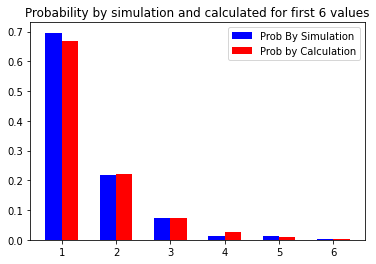
\includegraphics[scale=0.5]{img-1}
\end{center}




\end{multicols*}

\end{document}